% \iffalse
\let\negmedspace\undefined
\let\negthickspace\undefined
\documentclass[journal,12pt,twocolumn]{IEEEtran}
\usepackage{cite}
\usepackage{amsmath,amssymb,amsfonts,amsthm}
\usepackage{algorithmic}
\usepackage{graphicx}
\usepackage{textcomp}
\usepackage{xcolor}
\usepackage{txfonts}
\usepackage{listings}
\usepackage{enumitem}
\usepackage{mathtools}
\usepackage{gensymb}
\usepackage{comment}
\usepackage[breaklinks=true]{hyperref}
\usepackage{tkz-euclide} 
\usepackage{listings}
\usepackage{gvv}                                        
\def\inputGnumericTable{}                                 
\usepackage[latin1]{inputenc}                                
\usepackage{color}                                            
\usepackage{array}                                            
\usepackage{longtable}                                       
\usepackage{calc}                                             
\usepackage{multirow}                                         
\usepackage{hhline}                                           
\usepackage{ifthen}                                           
\usepackage{lscape}

\newtheorem{theorem}{Theorem}[section]
\newtheorem{problem}{Problem}
\newtheorem{proposition}{Proposition}[section]
\newtheorem{lemma}{Lemma}[section]
\newtheorem{corollary}[theorem]{Corollary}
\newtheorem{example}{Example}[section]
\newtheorem{definition}[problem]{Definition}
\newcommand{\BEQA}{\begin{eqnarray}}
\newcommand{\EEQA}{\end{eqnarray}}
\newcommand{\define}{\stackrel{\triangle}{=}}
\theoremstyle{remark}
\newtheorem{rem}{Remark}
\begin{document}

\bibliographystyle{IEEEtran}
\vspace{3cm}

\title{GATE: ST - 32.2023}
\author{EE22BTECH11039 - Pandrangi Aditya Sriram$^{*}$% <-this % stops a space
}
\maketitle
\newpage
\bigskip

\renewcommand{\thefigure}{\theenumi}
\renewcommand{\thetable}{\theenumi}


\vspace{3cm}
\textbf{Question:} Let $\cbrak{X_n}_{n \geq 1}$ be a sequence of independent and identically distributed random variables each having a mean $4$ and variance $9$. If $Y_n = \frac{1}{n} \sum_{i=1}^{n} X_i$ for $n \geq 1$, then $\lim\limits_{n \to \infty} \text{E}\sbrak{\brak{\frac{Y_n - 4}{\sqrt{n}}}^2}$ (in integer) equals \rule{2cm}{0.1mm}. \hfill(GATE ST 2023)
\\
\solution
% \fi
\begin{enumerate}
\item \textbf{Theory:}
For all $X_i$ which as i.i.d's, mean $\mu = 4$ and variance $\sigma^2 = 9$,
\begin{align}
    Y_n &= \frac{1}{n} \sum_{i=1}^{n} X_i
\end{align}
The mean of a sum of i.i.d random variables is calculated as
\begin{align}
    \text{E}\sbrak{Y_n} &= \text{E}\sbrak{\frac{1}{n} \sum_{i=1}^{n} X_i}\\
    &= \frac{1}{n} \sum_{i=1}^{n} \text{E}\sbrak{X_i}\\
    &= \frac{1}{n} (n\mu)\\
    &= \mu
\end{align}
The variance of a sum of i.i.d random variables is calculated as
\begin{align}
    \text{var}\brak{Y_n} &= \text{E}\sbrak{\brak{\frac{1}{n} \sum_{i=1}^{n} X_i}^2} - \brak{\text{E}\sbrak{\frac{1}{n} \sum_{i=1}^{n} X_i}}^2\\
    &= \frac{1}{n^2} \cbrak{\text{E}\sbrak{\brak{\sum_{i=1}^{n} X_i}^2} - \brak{\text{E}\sbrak{\sum_{i=1}^{n} X_i}}^2}\label{eq:st_32_2023_1}
\end{align}
But
\begin{align}
    \text{E}\sbrak{\brak{\sum_{i=1}^{n} X_i}^2} &= \text{E}\sbrak{\sum_{i=1}^{n} \sum_{j=1}^{n} X_iX_j}\\
    &= \sum_{i=1}^{n} \sum_{j=1}^{n} \text{E}\sbrak{X_iX_j} \label{eq:st_32_2023_2}
\end{align}
and 
\begin{align}
    \brak{\text{E}\sbrak{\sum_{i=1}^{n} X_i}}^2 &= \brak{\sum_{i=1}^{n} \text{E}\sbrak{X_i}}^2\\
    &= \sum_{i=1}^{n} \sum_{j=1}^{n} \text{E}\sbrak{X_i} \text{E}\sbrak{X_j} \label{eq:st_32_2023_3}
\end{align}
Putting \eqref{eq:st_32_2023_2} and \eqref{eq:st_32_2023_3} in \eqref{eq:st_32_2023_1}, and using the definition of covariance,
\begin{align}
    \text{var}\brak{Y_n} &= \frac{1}{n^2} \cbrak{\sum_{i=1}^{n} \sum_{j=1}^{n} \brak{\text{E}\sbrak{X_iX_j} - \text{E}\sbrak{X_i} \text{E}\sbrak{X_j}}}\\
    &= \frac{1}{n^2} \cbrak{\sum_{i=1}^{n} \sum_{j=1}^{n} \text{cov}\brak{X_i, X_j}} \label{eq:st_32_2023_4}
\end{align}
As all the variables are i.i.d's and are thus uncorrelated,
\begin{align}
    \text{cov}\brak{X_i, X_j} =
    \begin{cases}
        0 & \text{if } i \ne j\\
        \text{var}\brak{X_i} & \text{if } i = j
    \end{cases}\label{eq:st_32_2023_5}
\end{align}
Putting \eqref{eq:st_32_2023_5} in \eqref{eq:st_32_2023_4},
\begin{align}
    \text{var}\brak{Y_n} &= \frac{1}{n^2} \brak{\sum_{i=1}^{n} \text{cov}\brak{X_i, X_i}}\\
     &= \frac{1}{n^2} \brak{\sum_{i=1}^{n} \text{var}\brak{X_i}}\\
     &= \frac{1}{n^2} \brak{\sum_{i=1}^{n} \sigma^2}\\
     &= \frac{\sigma^2}{n}
\end{align}
Consider the term $\brak{\frac{Y_n - \mu}{\sqrt{n}}}^2$. Calculating its expectation,
\begin{align}
    \text{E}\sbrak{\brak{\frac{Y_n - \mu}{\sqrt{n}}}^2} &= \frac{1}{n} \text{E}\sbrak{\brak{Y_n - \mu}^2}\\
    &= \frac{1}{n} \text{var}\brak{Y_n}\\
    &= \frac{\sigma^2}{n^2}
\end{align}
Substituting $\sigma^2 = 9$ and $\mu = 4$, we get
\begin{align}
    \lim\limits_{n \to \infty} \text{E}\sbrak{\brak{\frac{Y_n - 4}{\sqrt{n}}}^2}
    = \lim\limits_{n \to \infty} \frac{9}{n^2} = 0 \label{eq:st_32}
\end{align}

\item \textbf{Simulation:}
Any distribution with mean $\mu = 4$ and variance $\sigma^2 = 9$ can be used for the variable $X_{ij}$ for all $i,j \in \mathbb{N}$; as shown in the Theory part, the limit is always zero regardless of the distribution. The most straightforward distribution that can be used for $X_{ij}$ is:
\begin{align}
    p_{X_{ij}}(x) = \begin{cases}
    0.5 &\text{if }x \in \cbrak{1, 7}\\
    0 &\text{otherwise }
    \end{cases}
\end{align}
This distribution has the following characteristics:
\begin{align}
    \mu &= \text{E}\sbrak{X_{ij}} = 0.5\times1 + 0.5\times 7 = 4\\
    \sigma^2 &= \text{E}\sbrak{X_{ij}^2} - \brak{\text{E}\sbrak{X_{ij}}}^2\\
    &= \brak{0.5 \times 1^2 + 0.5 \times 7^2} - 4^2\\
    &= 9
\end{align}
Alternatively, distributions such as $X_{ij} \sim \mathcal{N}(4, 9)$ could also be used. A matrix $X_{n \times m}$ is generated for all $i \leq n$ and $j \leq m$.
Using this matrix, a set of m values for $Y_j$ is generated as
\begin{align}
    Y_j = \frac{1}{n} \sum_{i = 1}^{n} X_{ij}
\end{align}
Now, the expression $\frac{\brak{Y_j - 4}^2}{n}$ is calculated for all $j \leq m$ and their expectancy is calculated as follows:
\begin{align}
    \text{E}\sbrak{\brak{\frac{Y_n - 4}{\sqrt{n}}}^2} &= \frac{1}{m}\sum_{j=1}^{m} \frac{\brak{Y_j - 4}^2}{n}
\end{align}
To calculate the limit $n \rightarrow \infty$, different values of n are taken, and the expected value is calculated (taking a fixed small value of m to reduce computational time) for each case. This output is plotted and is seen to be close to the curve $\frac{9}{n^2}$, as derived in \eqref{eq:st_32}. 
\begin{figure}[h!]
    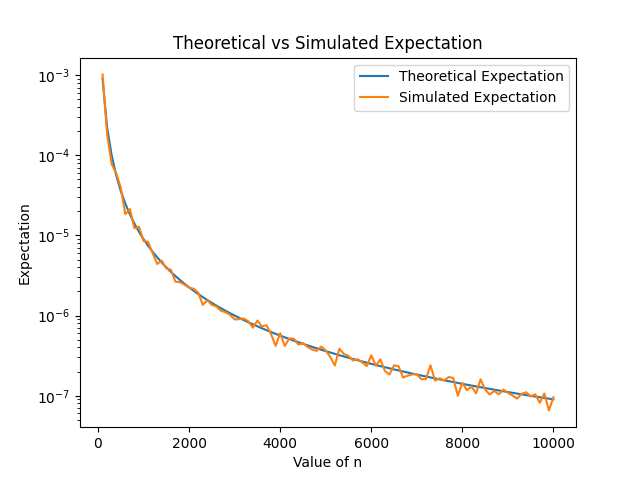
\includegraphics[width=\columnwidth]{figures/expectation.png}
    \caption{Expectation vs n}
    \label{fig:st_2023_32_figure}
\end{figure}
In both cases, we can observe the limit tends towards zero.
\end{enumerate}
\end{document}  